\section{Adaptive Element}
\label{s:network}
Single hidden layer (SHL) perceptron NNs are
universal approximators\cite{hornik_89,spooner,lewis:ajc:99}. Hence,
given a sufficient number of hidden layer neurons and appropriate
inputs, it is possible to train the network online to cancel model
error.
%
\begin{figure}[h]
  \centering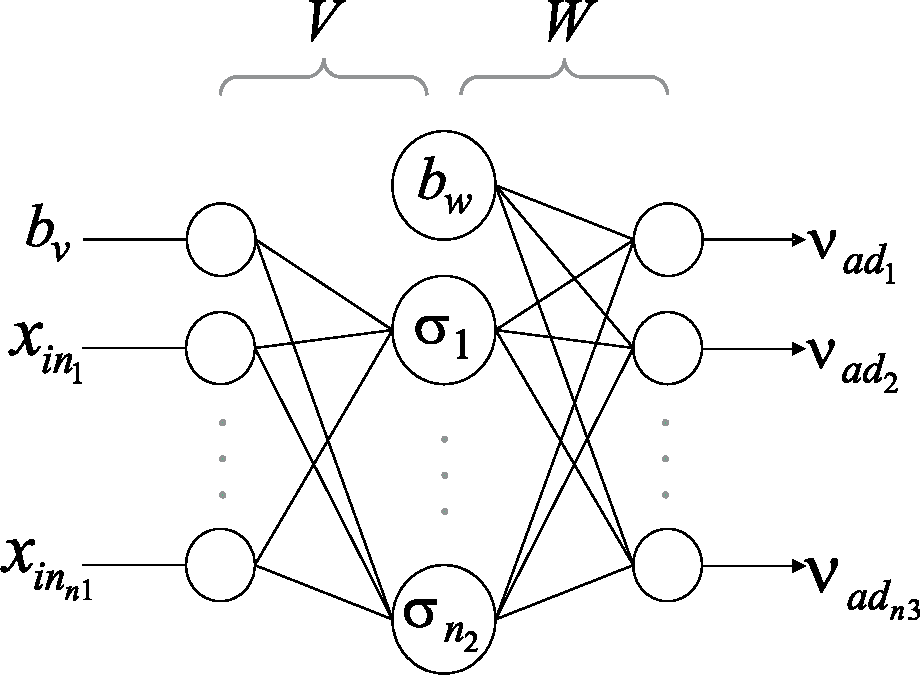
\includegraphics[width=.7\columnwidth]{nn}
%  \centering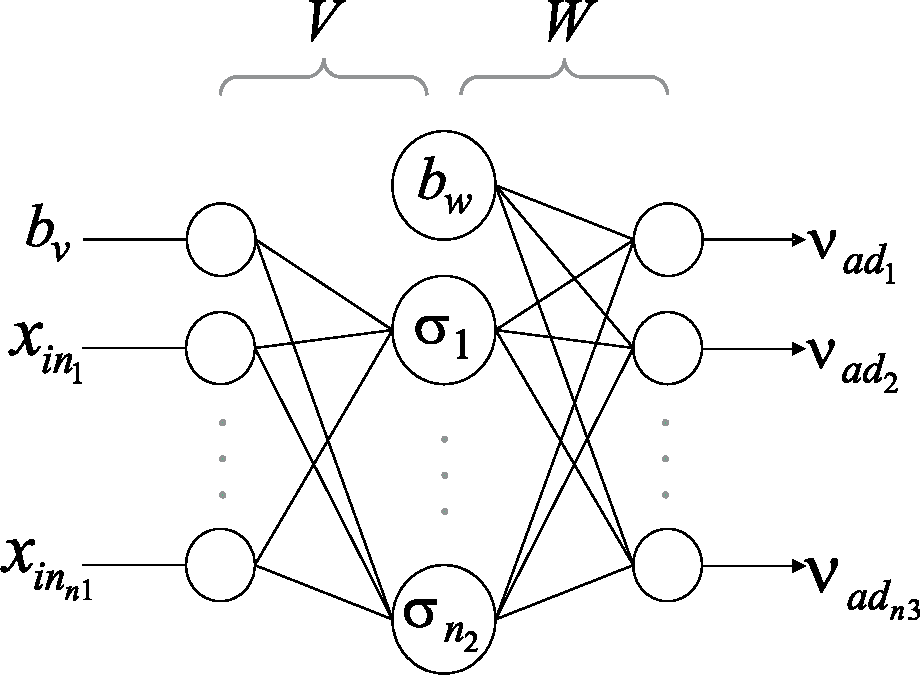
\includegraphics{nn}
  \caption{Neural Network with one hidden layer.}
  \label{f:nn}
\end{figure}
%
\fig{f:nn} shows the structure of a generic single hidden layer
network whose input-output map may be expressed as
\begin{equation}
\nu_{ad_k} = b_w\theta_{w_k} + \sum_{j=1}^{n_2}w_{jk}\sigma_j(z_j),
\end{equation}
where, $k=1,...,n_3$, $b_w$ is the outer layer bias,
$\theta_{w_k}$ is the $k^{th}$ threshold. $w_{jk}$ represents the
outer layer weights, $z_j$ is the input to the neurons, and the scalar $\sigma_j$ is a sigmoidal
activation function
\begin{equation}
\label{e:activation} \sigma_j(z_j) = \frac{1}{1 + e^{-az_j}},
\end{equation}
where, $a$ is the so called \emph{activation potential} and may
have a distinct value for each neuron. $z_j$ is the input to the
$j^{th}$ hidden layer neuron, and is given by
\begin{equation}
z_j = b_v\theta_{v_j} + \sum_{i=1}^{n_1}v_{ij}x_{in_i},
\end{equation}
where, $b_v$ is the inner layer bias and $\theta_{v_j}$ is the
$j^{th}$ threshold. Here, $n_1,n_2$ and $n_3$ are the number of
inputs, hidden layer neurons and outputs respectively. $x_{in_i},
i=1,...,n_1$, denotes the inputs to the NN. For convenience, define
the following weight matrices:
\begin{align}
V &\triangleq
\begin{bmatrix}
\theta_{v,1}    &     \cdots   & \theta_{v,n_2} \\
v_{1,1}         &     \cdots   & v_{1,n_2} \\
\vdots          &     \ddots   & \vdots \\
v_{n_1,1}       &     \cdots   & v_{n_1,n_2}
\end{bmatrix},  \\
W &\triangleq
\begin{bmatrix}
\theta_{w,1}    &     \cdots   & \theta_{w,n_3} \\
w_{1,1}         &     \cdots   & w_{1,n_3} \\
\vdots          &     \ddots   & \vdots \\
w_{n_2,1}       &     \cdots   & w_{n_2,n_3}
\end{bmatrix},  \\
\label{e:Z} Z &\triangleq
\begin{bmatrix}
V   &   0  \\
0   &   W
\end{bmatrix}.
\end{align}
%
Additionally, define the $\bfsigma(\bfz)$ vector as
\begin{equation}
\bfsigma^T(\bfz) \triangleq
\begin{bmatrix}
b_w    &    \sigma(z_1)  &  \cdots &  \sigma(z_{n_2}),
\end{bmatrix}
\end{equation}
where $b_w > 0$ allows for the thresholds, $\bftheta_w$, to be
included in the weight matrix $W$. Also, $\bfz = V^T\bar{\bfx}$,
where,
\begin{equation}
\bar{\bfx}^T =
\begin{bmatrix} b_v   & \bfx_{in}^T
\end{bmatrix},
\end{equation}
where, $b_v > 0$, is an input bias that allows for thresholds
$\bftheta_v$ to be included in the weight matrix $V$.
%
The input-output map of the SHL network may now be written in
concise form as
\begin{equation}
\label{e:nuad} \nuad = W^T\bfsigma(V^T\xbar).
\end{equation}
%
The NN may be used to approximate a nonlinear function, such as
$\Del(.)$. The universal approximation property\cite{hornik_89} of
NN's ensures that given an $\bar{\epsilon} > 0$, then $\forall$
$\xbar \in \domd$, where $\domd$ is a compact set, $\exists$ an
$\bar{n}_2$ and an ideal set of weights $(V^*,W^*)$, that brings the
output of the NN to within an $\epsilon$-neighborhood of the
function approximation error. This $\epsilon$ is bounded by
$\bar{\epsilon}$ which is defined by
\begin{equation}
\bar{\epsilon} = \sup_{\xbar \in \domd} \left\|
W^T\bfsigma(V^T\xbar) - \Del(\xbar) \right\|.
\end{equation}
The weights, $(V^*,W^*)$ may be viewed as optimal values of $(V,W)$
in the sense that they minimize $\bar{\epsilon}$ on $\domd$. These
values are not necessarily unique. The universal approximation
property thus implies that if the NN inputs $\bfx_{in}$ are chosen
to reflect the functional dependency of $\Del(\cdot)$, then
$\bar{\epsilon}$ may be made arbitrarily small given a sufficient
number of hidden layer neurons, $n_2$.

\begin{comment}
\subsubsection{Instantaneous update laws}
 Define $r=e^TPB$, where $P$ is the positive definite solution to the Lyapunov equation as defined in \ref{eq:Lyap}
    \begin{eqnarray}
    \label{eq:backprop_shl}
    \dot{W}=-(\sigma(\bar x)-\sigma'(V^T\bar{x})V^T\bar{x}) r^T \Gamma_W,\\
    \label{eq:backprop_shl_V}
    \dot{V} =  - \Gamma _V \bar xr^TW^T \sigma'(V^T\bar{x}),
    \end{eqnarray}
    where $\Gamma_W,\Gamma_V$ are positive definite matrices that define the learning rate of the NN. This update law closely resembles the backpropagation method of tuning NN weights \cite{Rumelhart:86Nature,Suykens:96bk,Haykin:98bk,Kim:98bk}. However, it is important to note that the training signal $r$ is different from that of the backpropagation based learning laws \cite{Kim:98bk}.
    \end{comment}

